% Created 2016-10-13 jue 18:16
\documentclass[11pt]{article}
\usepackage[utf8]{inputenc}
\usepackage[T1]{fontenc}
\usepackage{fixltx2e}
\usepackage{graphicx}
\usepackage{longtable}
\usepackage{float}
\usepackage{wrapfig}
\usepackage{rotating}
\usepackage[normalem]{ulem}
\usepackage{amsmath}
\usepackage{textcomp}
\usepackage{marvosym}
\usepackage{wasysym}
\usepackage{amssymb}
\usepackage{hyperref}
\tolerance=1000
\usepackage[T1]{fontenc}
\usepackage[margin=2.5cm,includefoot]{geometry}
\usepackage{graphicx}
\usepackage{pict2e}
\usepackage{amsmath}
\usepackage{chngcntr}
\usepackage{hyperref}
\usepackage{import}
\hypersetup{colorlinks,citecolor=green,filecolor=black,linkcolor=blue,urlcolor=blue}
\author{Jorge Timón}
\date{\today}
\title{libconsensus}
\hypersetup{
  pdfkeywords={Bitcoin, consensus, libconsensus, libbitcoinconsensus},
  pdfsubject={},
  pdfcreator={Emacs 24.5.1 (Org mode 8.2.10)}}
\begin{document}

\maketitle
\tableofcontents


\setcounter{secnumdepth}{5}
\counterwithin{figure}{section}
\setcounter{tocdepth}{5}

\begin{abstract}
In Bitcoin (a distributed consensus system), there's a set of rules
which define whether a block is valid or not. In a typical software
system, those rules would be described in a specification document
written in a natural language that would then be translated to
one or more software implementations. But since software deployment
coordination is critical to the security of the system when the
software validation of the rules is changed, the documentation
doesn't necessarily have preference over the deployed implementation
when it comes to what is the specification to follow.

This produces an unnecessary network effect in favor of the
implementation deployed more widely, in this case, Bitcoin Core. Not
all of bitcoin is consensus critical, there's network messages,
storage, local relay and mining policies, wallet-specific code, code
specific to maintain indexes, GUI specific code...
This puts alternative implementations in an unnecessarily complicated
position when it comes to review and upgrade for changes to the
consensus rules.

Even if Bitcoin Core was adverse to the existence of alternative full-node implementations,
encapsulating consensus-critical code is necessary and urgent for
Bitcoin Core because it will enormously increase the number of potential
contributions to the project by drastically reducing the
probabilities that one particular change needs to touch any file
containing consensus-critical code and therefore reduce the demand for critical review. 

At the same time, the attack surface area of a bitcoin node is big, and
this sometimes leads to necessary complexity in the code to protect a
node from different potential attacks. These complexities must be
kept separated from the specification of the consensus rules of the
chain. 
But experience shows us that in the case of distributed consensus
systems like Bitcoin, for the specification to be truly unambiguous it
needs to be written directly in code.

Since Bitcoin Core is currently the more widely adopted full-node implementation, it makes sense to exact the first it from 
\end{abstract}

\newpage
\section{{\bfseries\sffamily TODO} Motivation}
\label{sec-1}

This document describes a detailed plan to separate consensus critical code from Bitcoin Core.


 to be able to give
reasonable guarantees that the same specification will be exactly
replicated by all nodes (that want to replicate it, see BIP99 for a
classification of potential changes to the specification) These nodes
may be implemented and integrated in diverse stacks with diverse machines.
A common specification of the consensus rules is necessary (but not
sufficient) for all participant to converge on the same view of the
history of global states of the system. But this specification is
currently coupled with Bitcoin Core's implementation of a full node,
which reduces its clarity and ease of modification.

Additionally, alternative implementations of the consensus protocol
are currently forced to chose between providing an incomplete full
node and relying on trusted nodes using the reference implementation
(Bitcoin Core)

Matt Corallo came up with the idea of exposing the newly encapsulated\ldots{}TODO

\newpage
\section{Current situation}
\label{sec-2}

In 0.13, Bitcoin core is divided in the following basic packages:

\begin{verbatim}
LIBBITCOIN_SERVER=libbitcoin_server.a
LIBBITCOIN_COMMON=libbitcoin_common.a
LIBBITCOIN_CONSENSUS=libbitcoin_consensus.a
LIBBITCOIN_CLI=libbitcoin_cli.a
LIBBITCOIN_UTIL=libbitcoin_util.a
LIBBITCOIN_CRYPTO=crypto/libbitcoin_crypto.a
LIBBITCOINQT=qt/libbitcoinqt.a
LIBSECP256K1=secp256k1/libsecp256k1.la
LIBBITCOIN_ZMQ=libbitcoin_zmq.a
LIBBITCOIN_WALLET=libbitcoin_wallet.a
\end{verbatim}

The figure \ref{pic_1_current} contains a simplified UML components diagram of
the current structure of Bitcoin Core, showing the executable
binaries as interfaces 

\begin{figure}[htb]
\centering
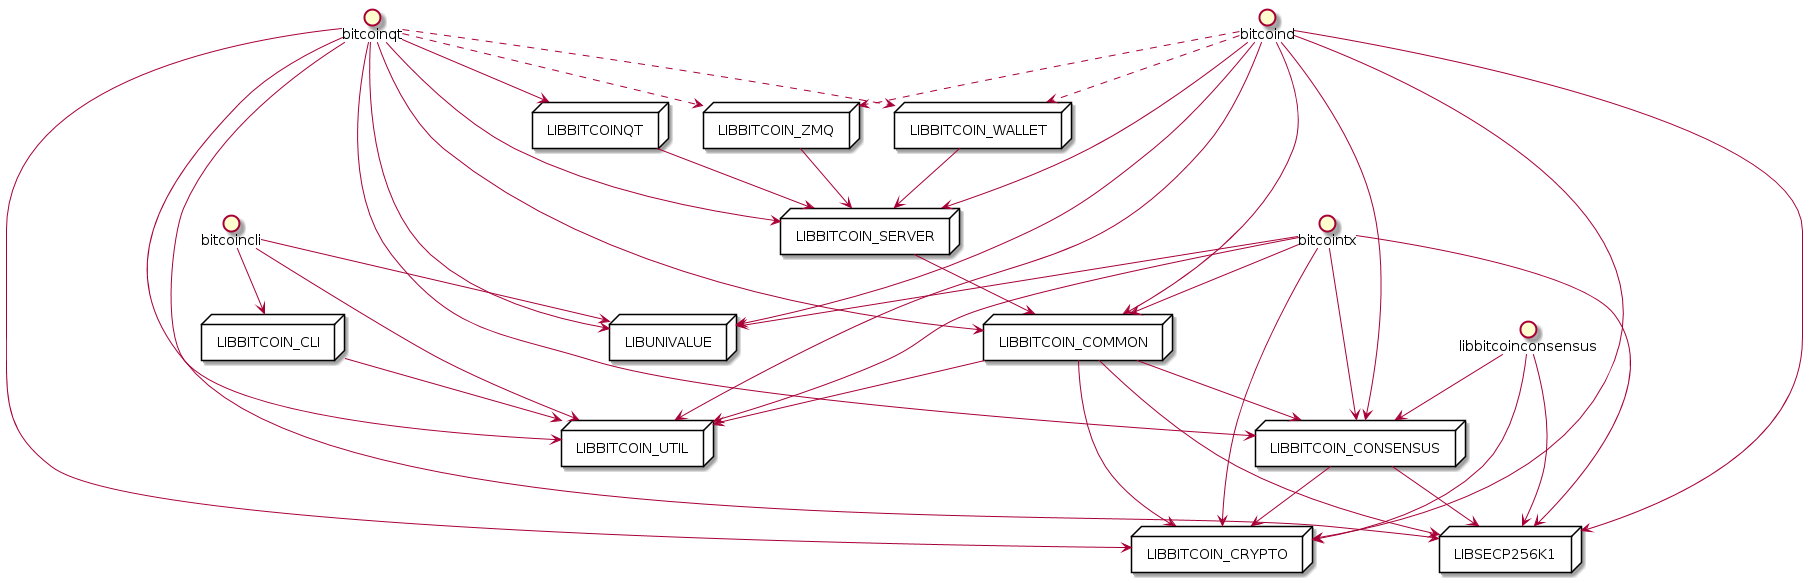
\includegraphics[width=.9\linewidth]{./img/1_current.png}
\caption{\label{pic_1_current}Current Bitcoin Core architecture}
\end{figure}

The arrows mean dependencies. The dotted discontinuous arrows mean
that the dependency can optionally be removed at compile time (it's
only used for \texttt{LIBBITCOIN\_WALLET} and \texttt{LIBBITCOIN\_ZMQ}, which are optional to both bitcoind
and bitcoin-qt).

Since some dependencies are implicit, we can remove some arrows to
simplify things as shown in figure \ref{pic_2_current_less_arrows}.

\begin{figure}[htb]
\centering
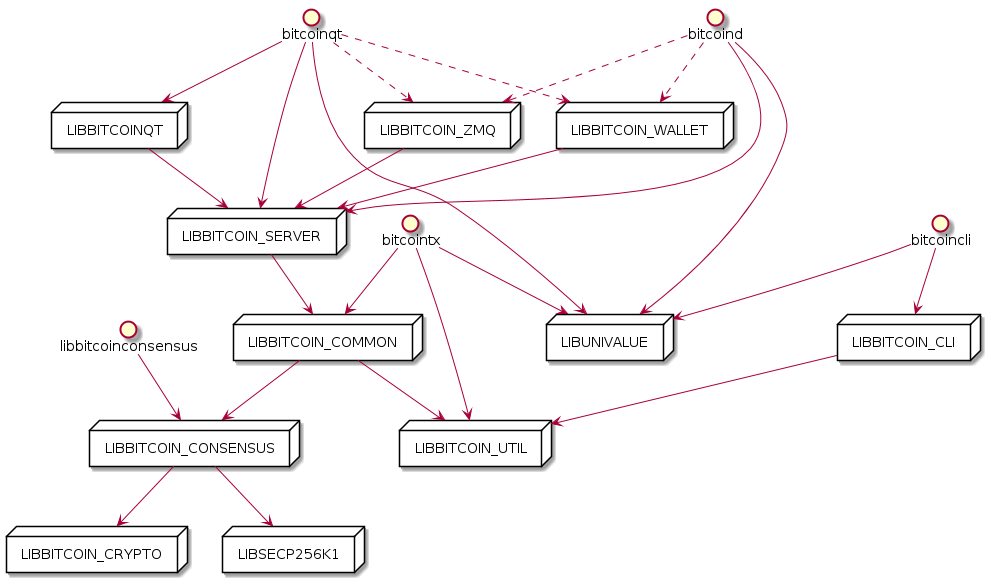
\includegraphics[width=.9\linewidth]{./img/2_current_less_arrows.png}
\caption{\label{pic_2_current_less_arrows}Simplified Current Bitcoin Core architecture}
\end{figure}

Also, bitcoin-cli, bitcoin-qt, \texttt{LIBBITCOIN\_ZMQ} and \texttt{LIBBITCOIN\_WALLET} are
encapsulated enough while not being too relevant to libconsensus that
we can remove them from the picture (see figure \ref{pic_3_current_simpler}).

\begin{figure}[htb]
\centering
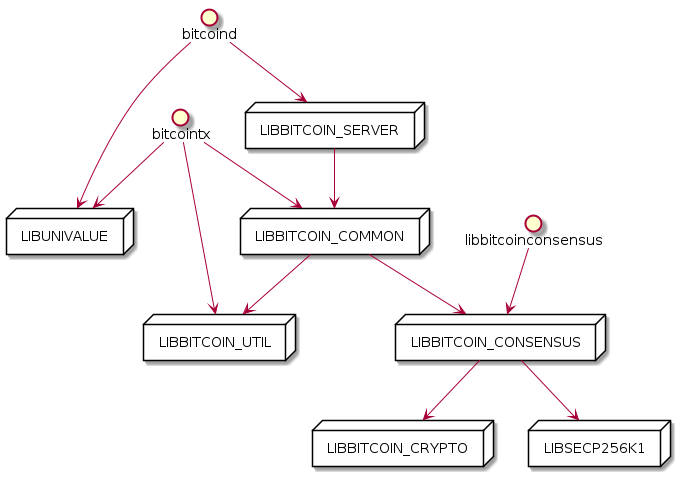
\includegraphics[width=.9\linewidth]{./img/3_current_simpler.png}
\caption{\label{pic_3_current_simpler}Simplified Current Bitcoin Core architecture excluding cli, qt, zmq and wallet.}
\end{figure}

libbitcoinconsensus currently only exposes \texttt{VerifyScript()}. We will
refer to all the previous work, including exposing \texttt{VerifyScript()}
(see PR \#4692 and its replacement \#5235) and other preparations up to
0.13 as "phase 1". After phase 1, we actually have some code we can
call libconsensus.

Before discussing phase 2, it is convenient to detail the current
state further, including concrete files within the packages as shown
in figure \ref{pic_4_current_libconsensus}.
The consensus package already contains more files than are needed for
\texttt{VerifyScript()}, but which contain mostly consensus code without also
including globals or undesired dependencies that would break
libconsensus. Those files are marked as green. Files marked as red
contain consensus critical code but cannot be added to the consensus
packages because they contain storage related dependencies or more
code that should not be moved to libconsensus (main.o, chain.o,
coins.o, pow.o and versionbits.o). Files marked with orange require
further discussion.

\begin{figure}[htb]
\centering
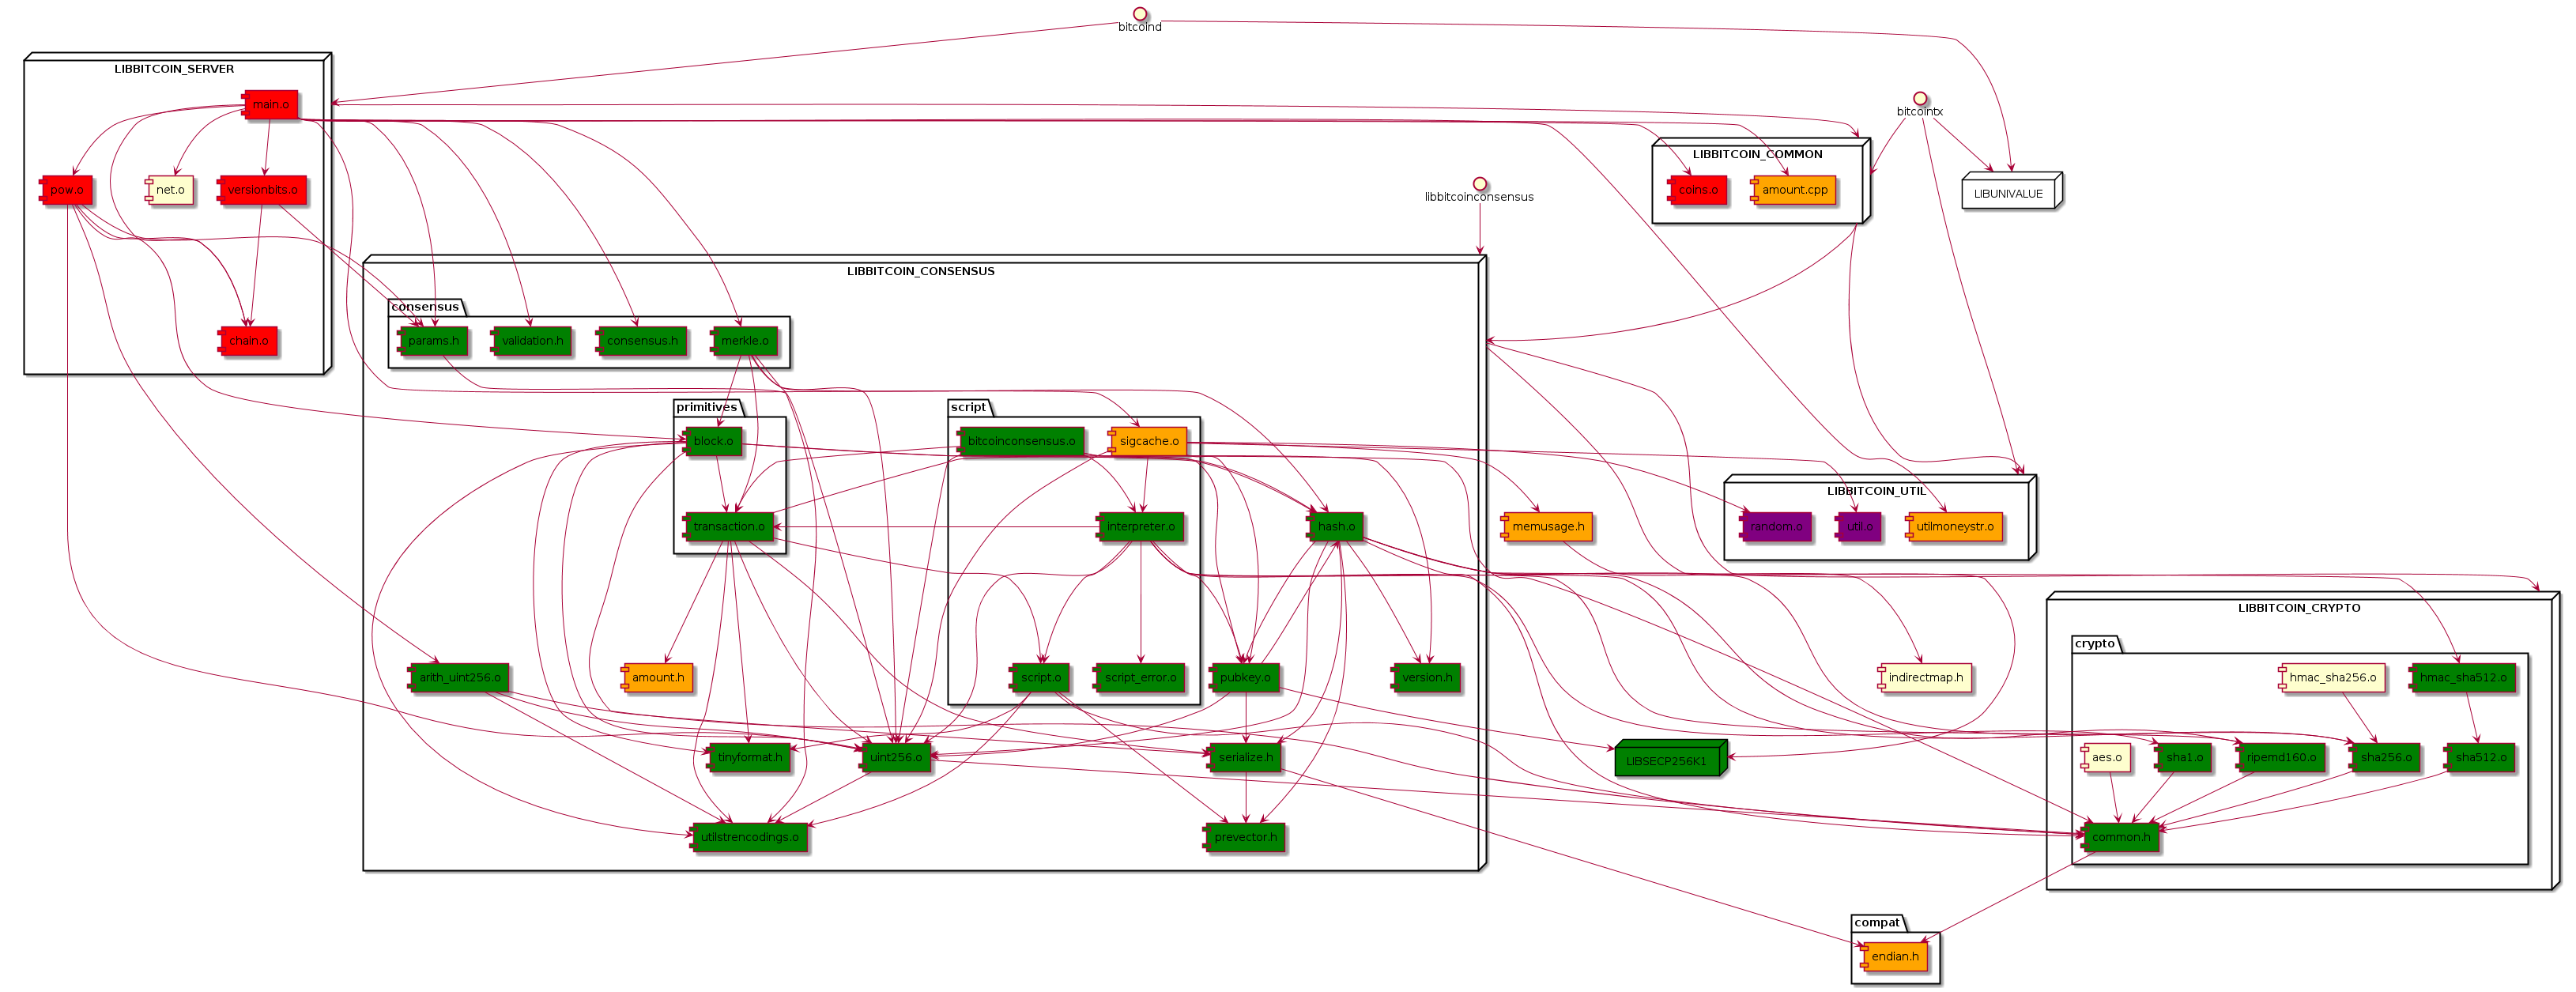
\includegraphics[width=.9\linewidth]{./img/4_current_libconsensus.png}
\caption{\label{pic_4_current_libconsensus}Detail of the current state of libconsensus}
\end{figure}

For example, amount.h is necessary for libconsensus, but it contains
CFeeRate, which should be moved out of the consensus packages.
CFeeRate is defined in amount.cpp, which is currently \textbf{not} used by
the consensus packages. This situation can be resolved by moving the
class CFeeRate to its own module, for example, policy/feerate.o as in
PR \#7820.

The only consensus function that uses utilmoneystr.o is
\texttt{Consensus::CheckTxInputs()}, currently in main.o. If the amounts in
some errors in that functions are shown in satoshis instead of
formatting them to full bitcoins using \texttt{FormatMoney()}, then
utilmoneystr.o doesn't need to be in the consensus package.

If we don't want to have compat/endian.h in libbitcoinconsensus,
crypto/common.h and seralize.h need to be decoupled from it.

If we want to include script/sigcache.o in the the consensus library,
we need to consider its dependency memusage.h and decouple it from
random.o and util.o.

\newpage
\section{Phase 2: Expose \texttt{VerifyHeader()}}
\label{sec-3}

As a next function to expose in libconsensus, we can use
\texttt{VerifyHeader()}. Although it relies on chain storage (\texttt{CBlockIndex}
class in Bitcoin Core), it is probably the simplest verify function to
expose. SPV wallets could call this functions for fully verifying the
header (including difficulty adjustments) instead of only checking the proof of work.

Since we want libbitcoinconsensus to be independent of the storage,
CBlockIndex needs to be replaced with some sort of interface
compatible with libconsensus' C API. For example, \#8493 introduces a C
struct \texttt{BlockIndexInterface} containing function pointers as fields. These functions are
used to access the header index. For libconsensus, each header is just
a void pointer used only with the help of \texttt{BlockIndexInterface}. Since
each caller may have a different structure for their header object, we
cannot assume any particular one and we take them as void pointers.

To move the header validation functions and their dependency pow.o to
the consensus package, we need to decoupled the from chain.o (where
\texttt{CBlockIndex} is defined) using this interface. Figure
\ref{pic_5_phase2} shows the result of applying phase 2.

\begin{figure}[htb]
\centering
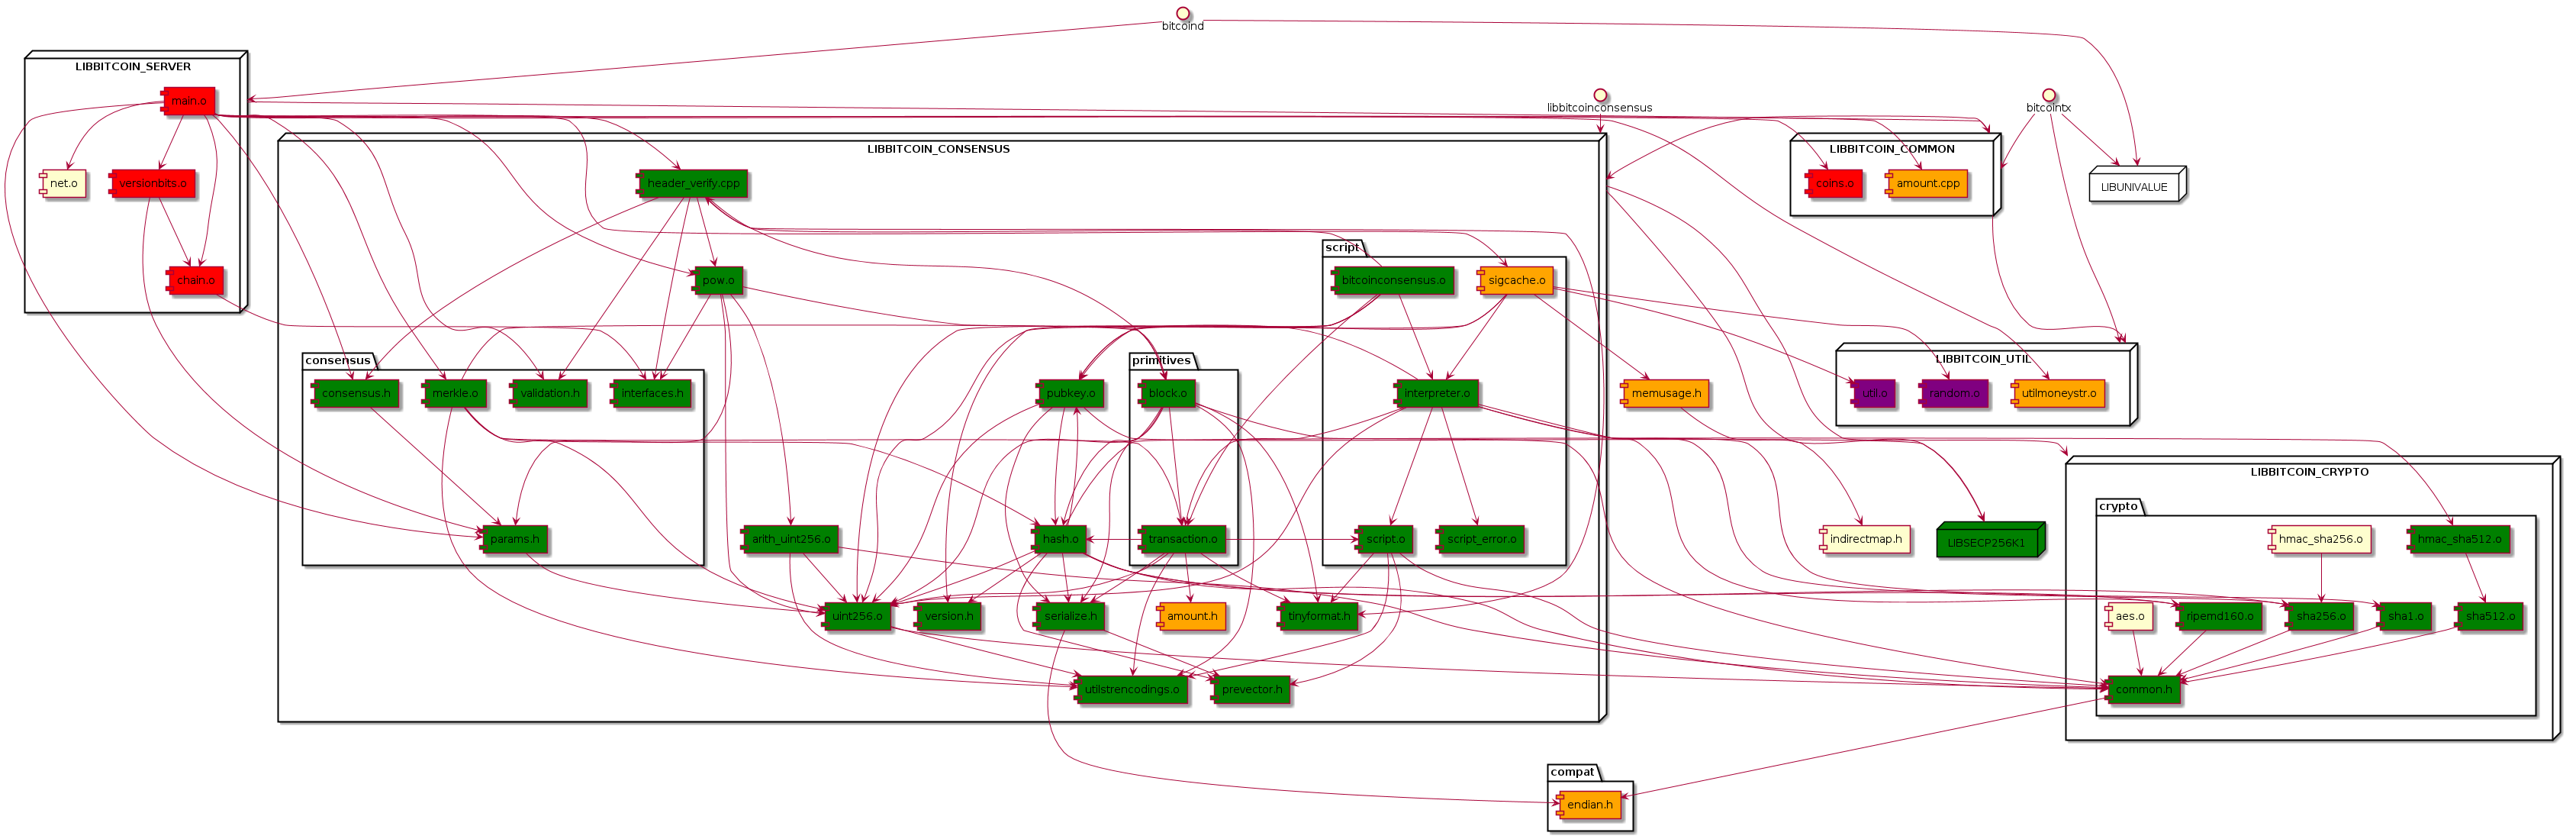
\includegraphics[width=.9\linewidth]{./img/5_phase2_libconsensus.png}
\caption{\label{pic_5_phase2}Phase 2: Expose \texttt{VerifyHeader()}}
\end{figure}

\newpage
\section{{\bfseries\sffamily TODO} Phase 3: Expose \texttt{GetConsensusFlags()}}
\label{sec-4}

\begin{figure}[htb]
\centering
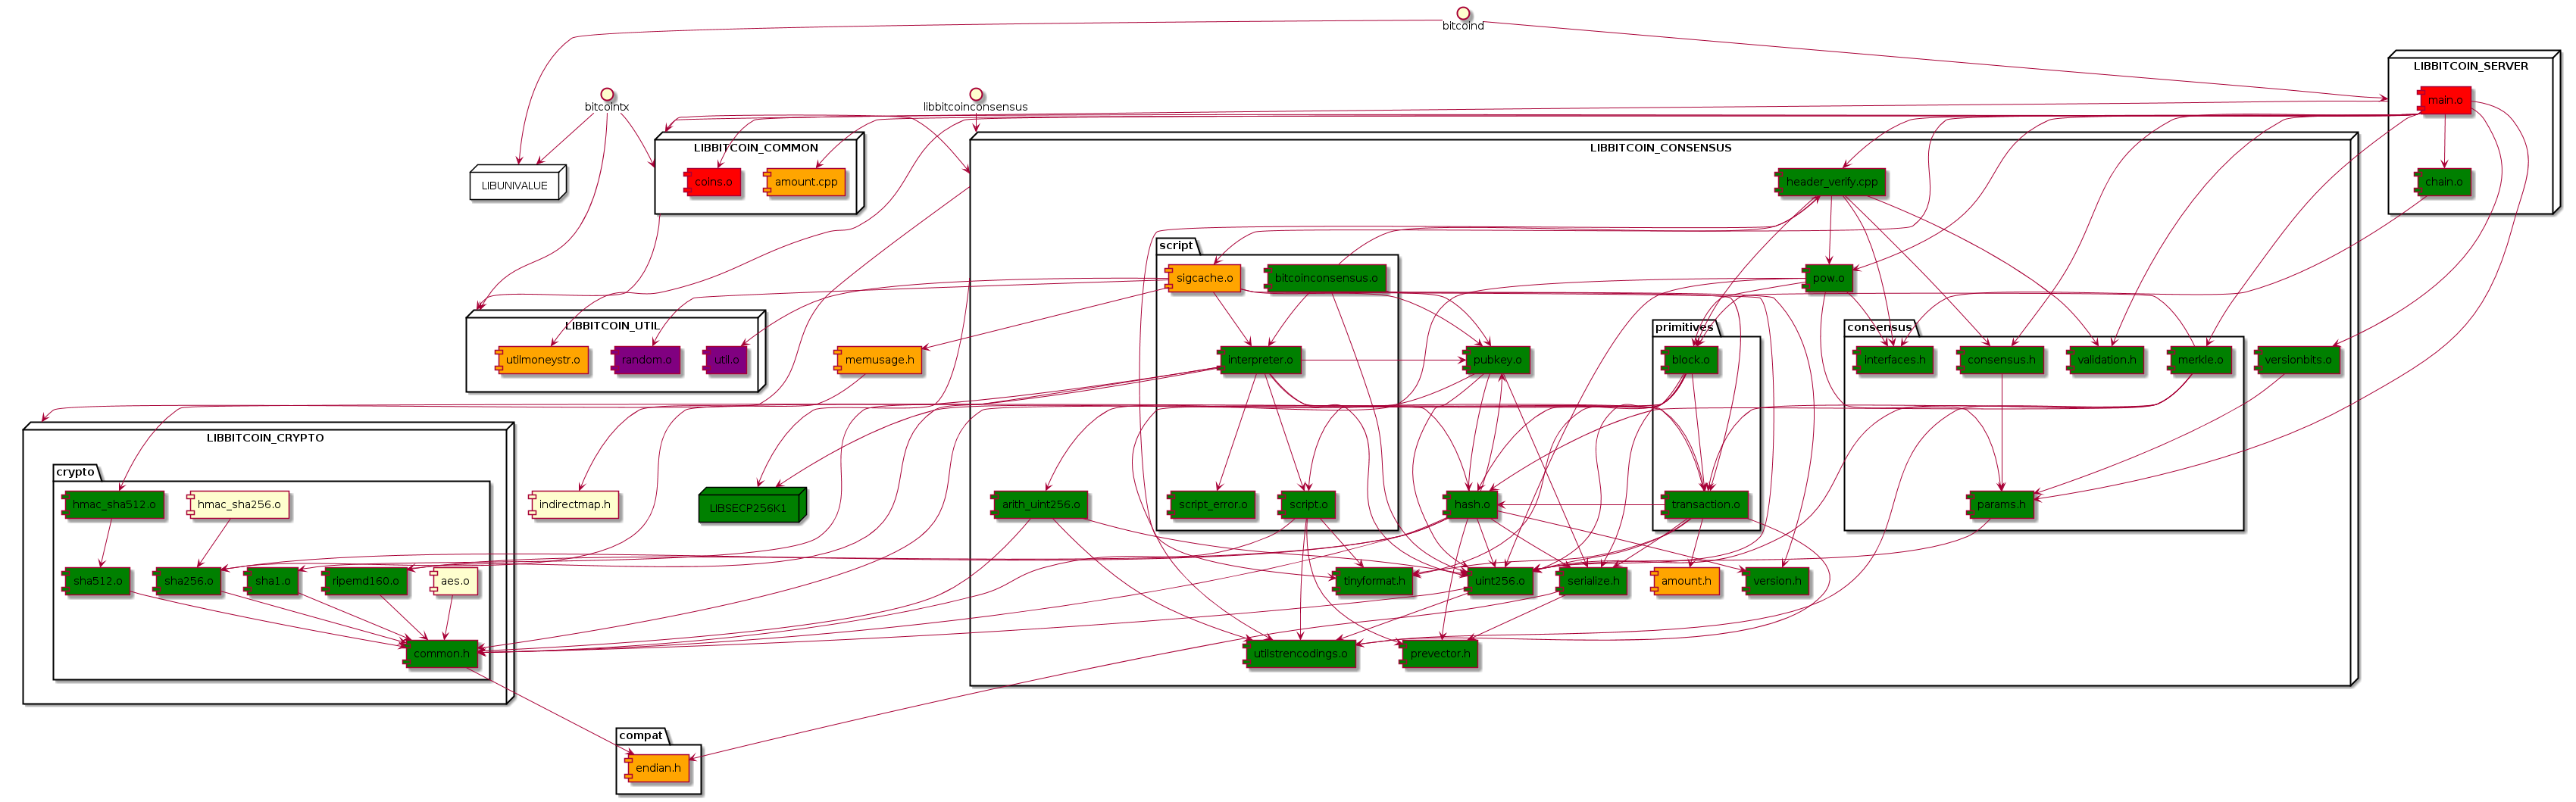
\includegraphics[width=.9\linewidth]{./img/6_phase3_libconsensus.png}
\caption{\label{pic_6_phase3}Phase 3: Expose \texttt{GetConsensusFlags()}}
\end{figure}

\newpage
\section{{\bfseries\sffamily TODO} Phase 4: Expose \texttt{VerifyTx()}}
\label{sec-5}

\begin{figure}[htb]
\centering
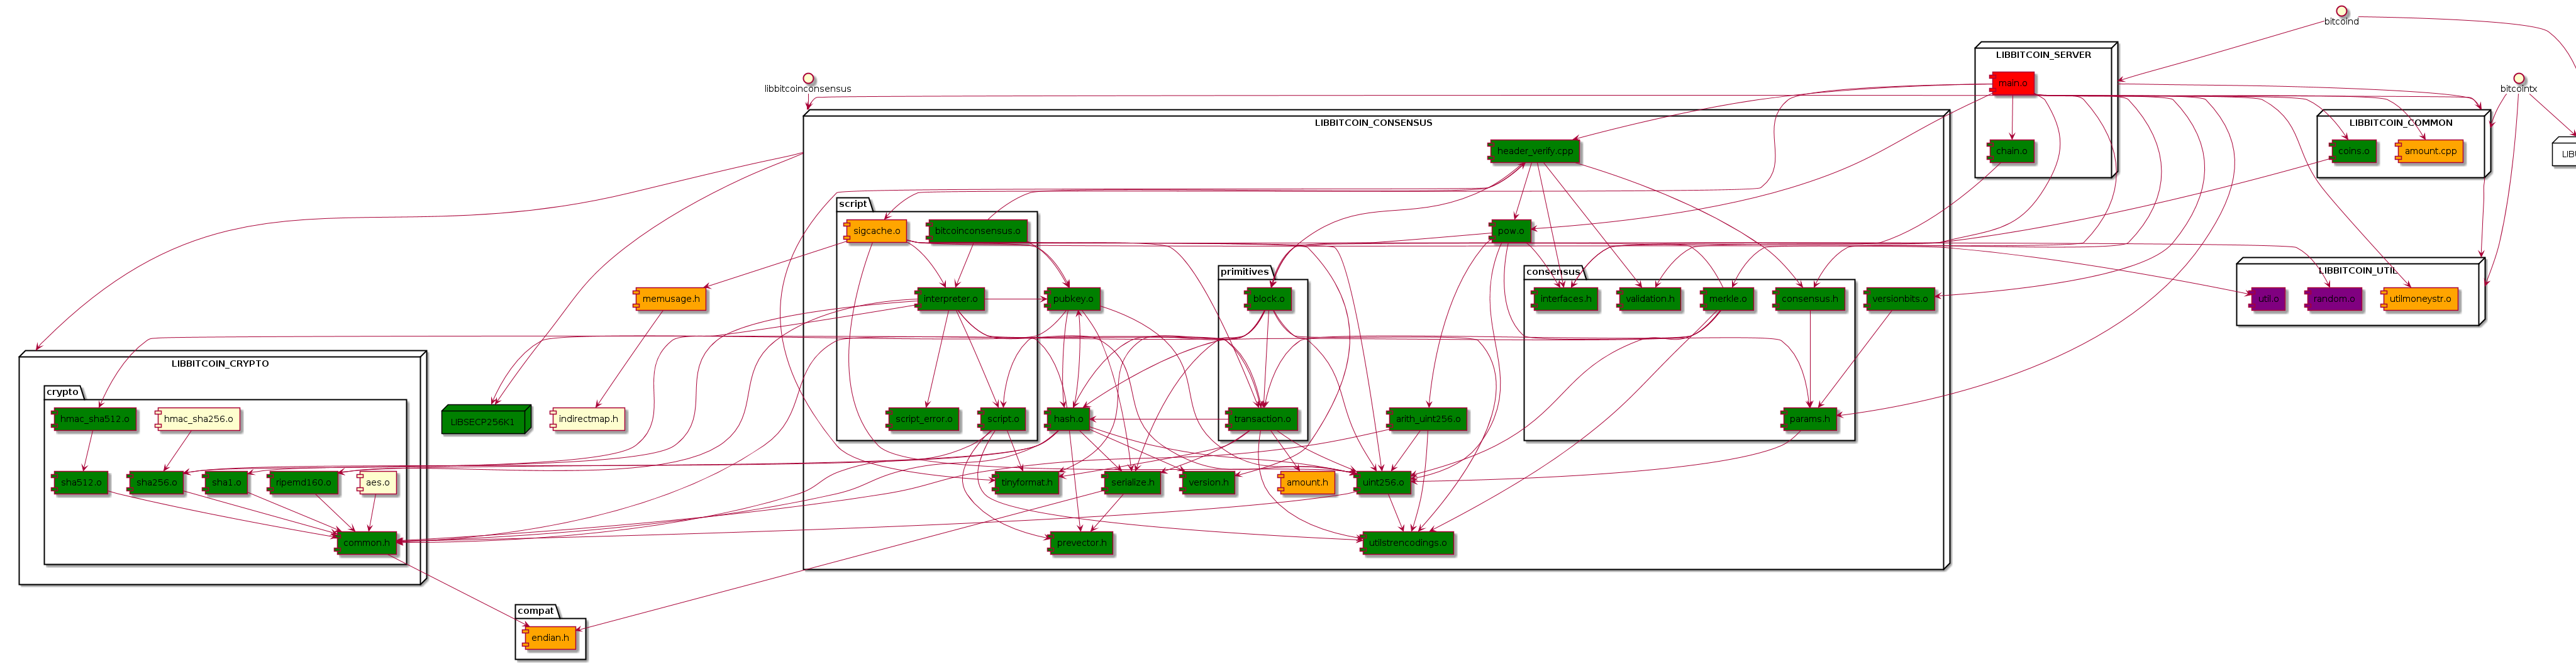
\includegraphics[width=.9\linewidth]{./img/7_phase4_libconsensus.png}
\caption{\label{pic_7_phase4}Phase 4: Expose \texttt{VerifyTx()}}
\end{figure}

\newpage
\section{{\bfseries\sffamily TODO} Phase 5: Complete libconsensus API (expose \texttt{VerifyBlock()})}
\label{sec-6}

\begin{figure}[htb]
\centering
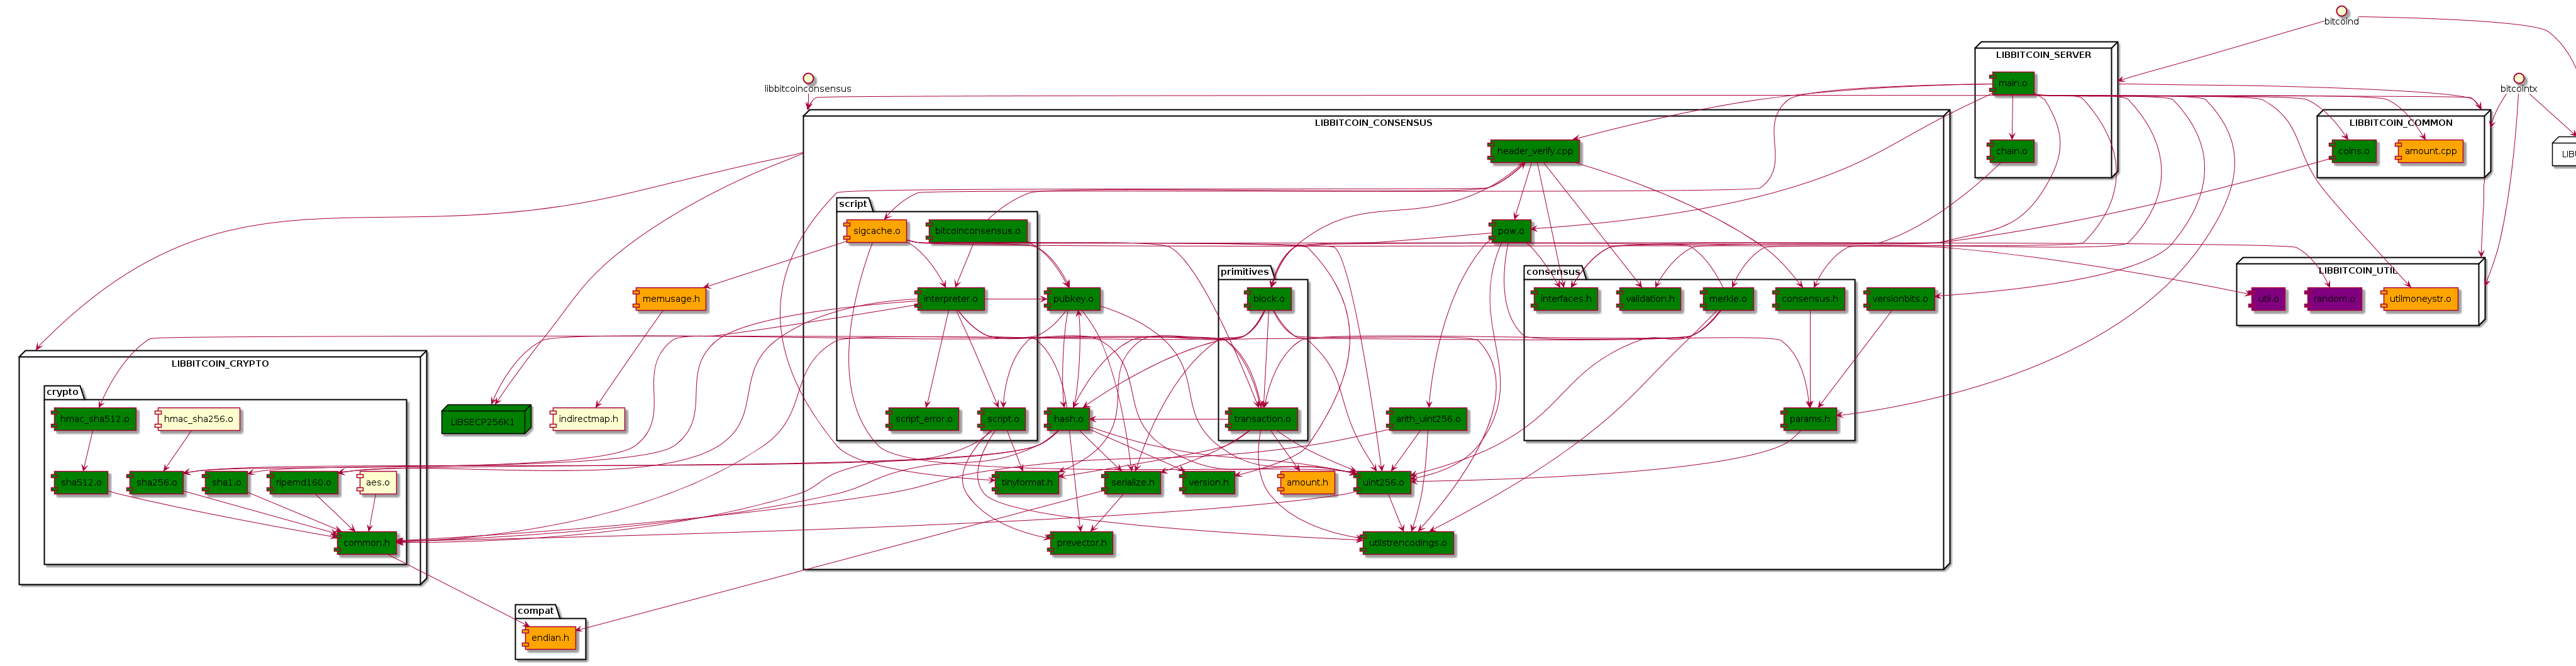
\includegraphics[width=.9\linewidth]{./img/8_phase5_libconsensus.png}
\caption{\label{pic_8_phase5}Phase 5: Expose \texttt{VerifyBlock()}}
\end{figure}

\newpage
\section{{\bfseries\sffamily TODO} Phase 6: Separate libconsensus to its own repository}
\label{sec-7}
\subsection{Phase 6.1: Remove non-consensus code.}
\label{sec-7-1}
\subsection{Phase 6.2: Move all consensus code to the same directory}
\label{sec-7-2}
\subsection{Phase 6.3: Create a sub-repository or subtree}
\label{sec-7-3}

\begin{figure}[htb]
\centering
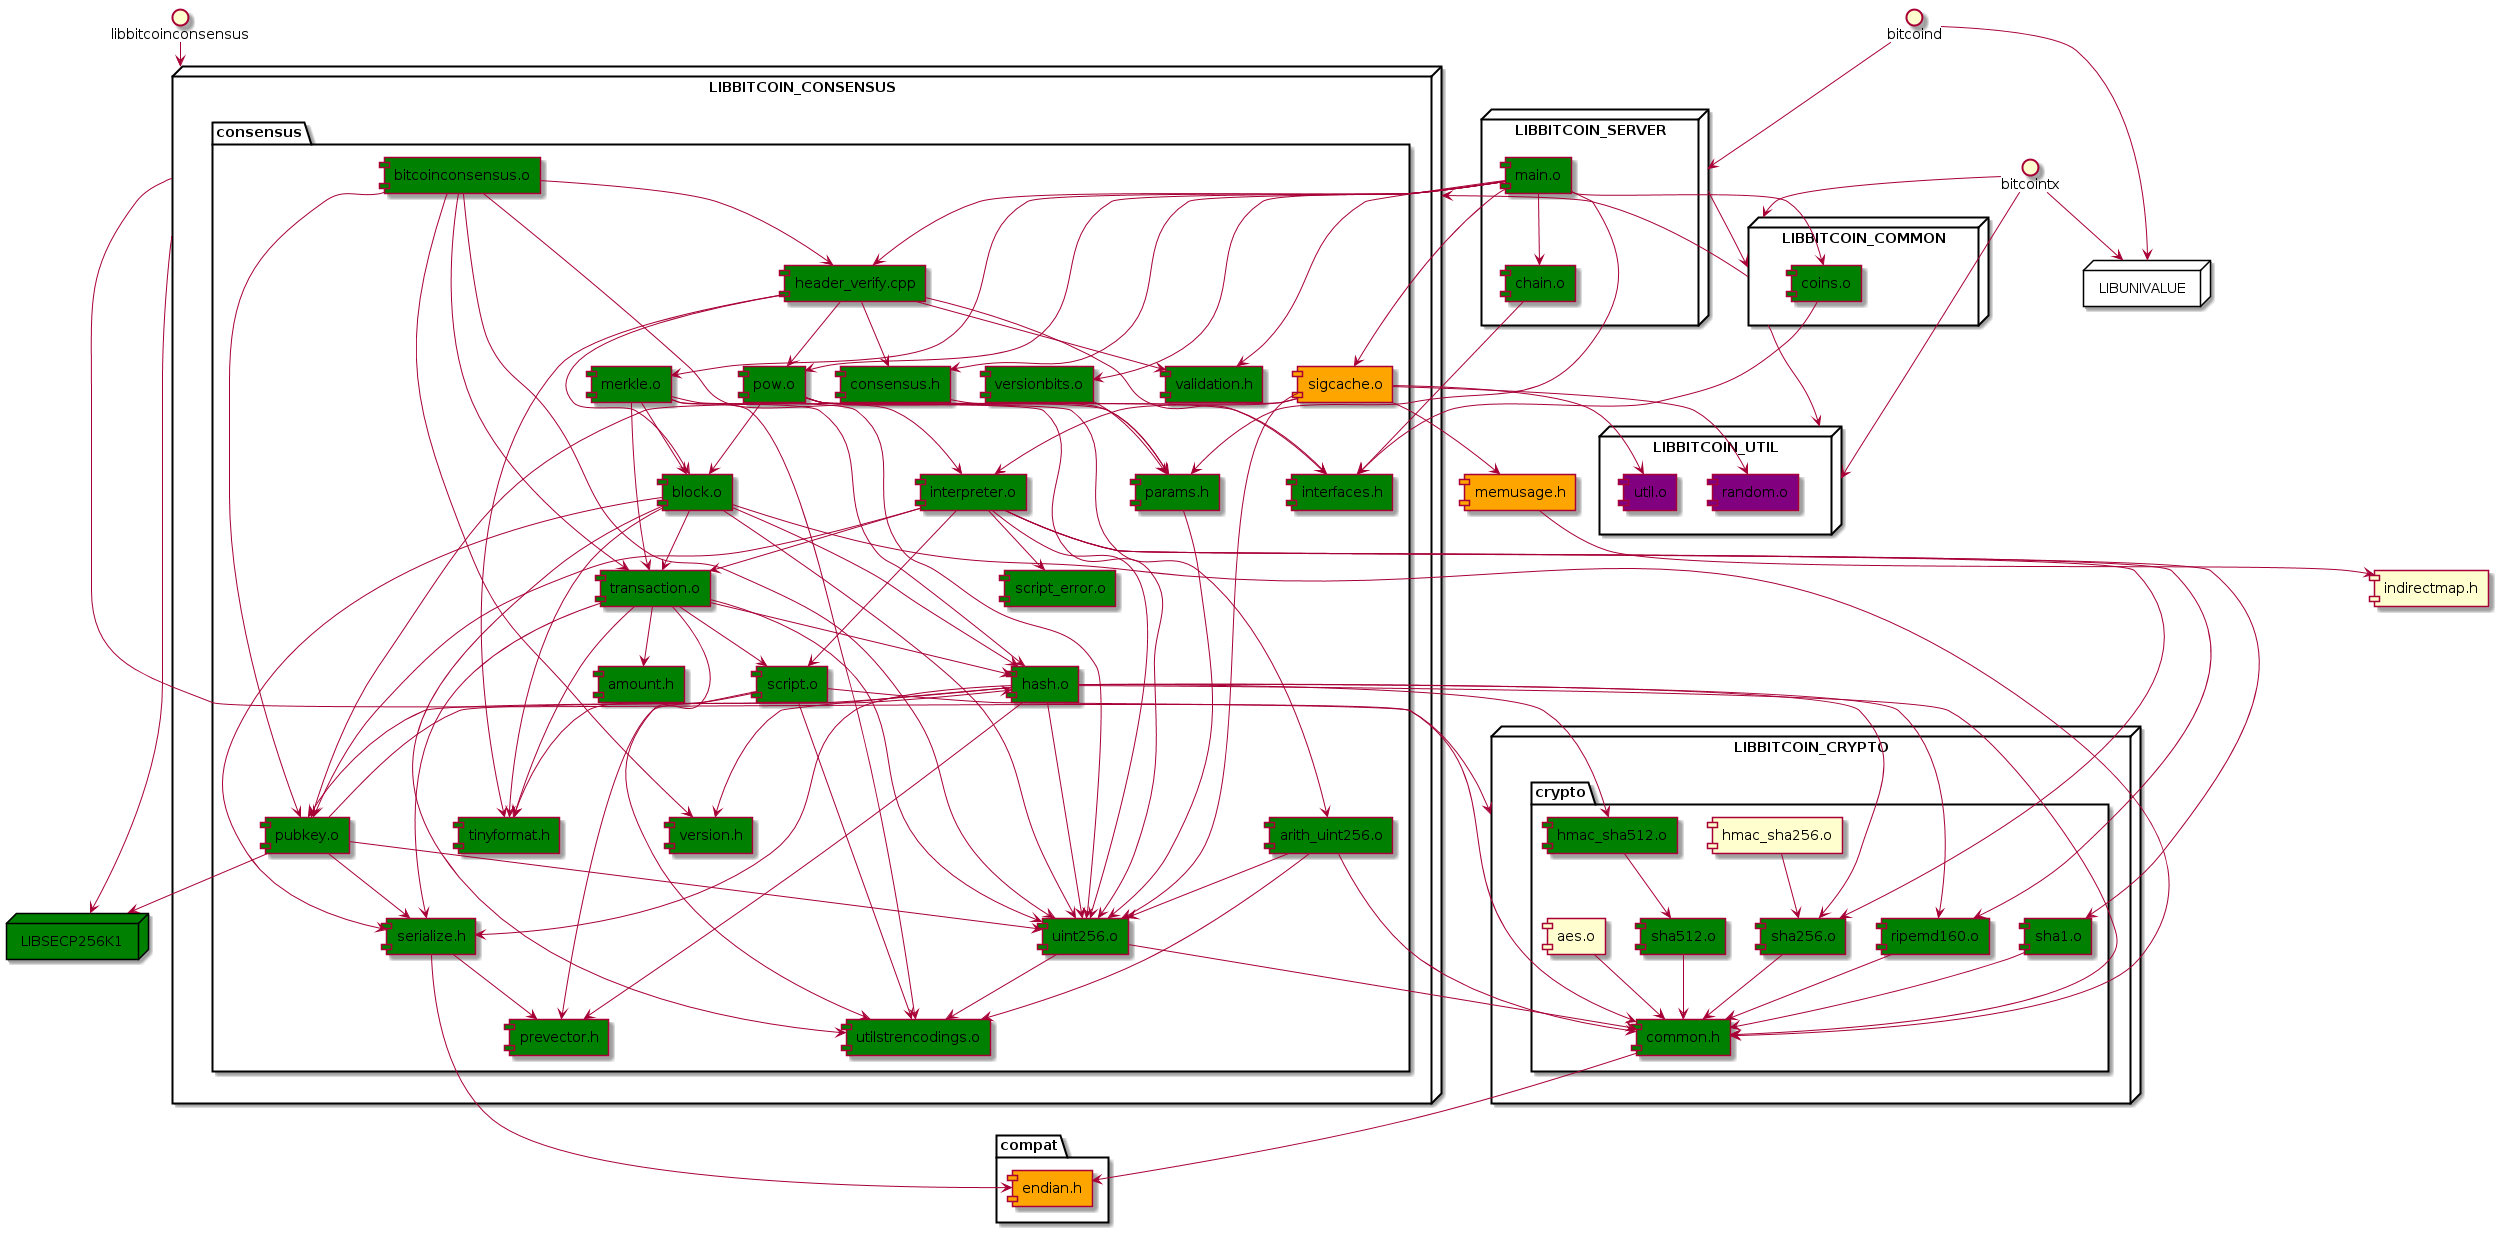
\includegraphics[width=.9\linewidth]{./img/9_phase6_libconsensus.png}
\caption{\label{pic_9_phase6}Phase 6: Separate libconsensus to its own repository}
\end{figure}

\newpage
\section{{\bfseries\sffamily TODO} Phase 7: Make Bitcoin Core eat its own dog food}
\label{sec-8}
\newpage
\section{{\bfseries\sffamily TODO} Final proposed complete libconsensus' C API}
\label{sec-9}
\newpage
% Emacs 24.5.1 (Org mode 8.2.10)
\end{document}
